\section{Public Methods}

These methods can be used by all \cpp\ -programs that have included
the header file {\em ChromosomeT.h} and the library {\em EA}.

\subsection{Mutation Methods}

\subsection{Random Number Distribution for Mutation Methods}

The following mutation methods will use a special kind of
distribution function for the random numbers, that was
developed especially for integer numbers.
The normal Gaussian distribution for continuous random numbers
produces no satisfactory output for integer values, because
the necessary rounding distorts the results. 
For this reason the methods in the {\tt integer} class
use a distribution as depicted in figure \ref{verteilung}.
By using a step size {\em s} the distribution of the
random numbers can be influenced. The greater {\em s} is,
the ``wider'' will be the distribution of the random numbers.

\begin{figure}[ht]
    \vspace*{-30ex}
    \centerline{
        \hfill
        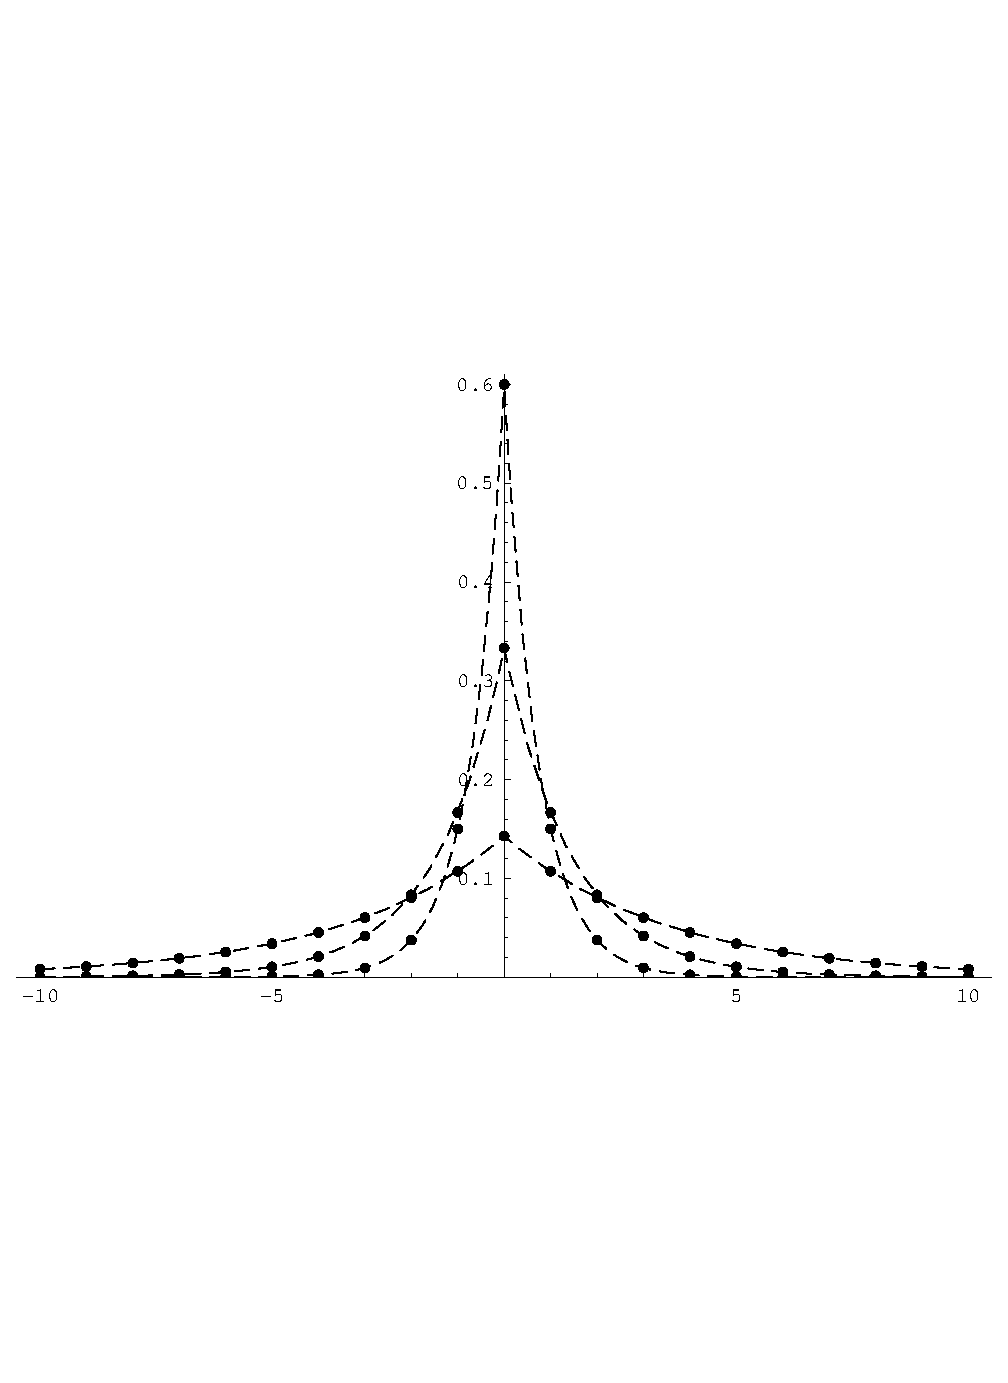
\includegraphics[width=\textwidth]{diffGeom.eps}
        \hfill
    }
    \vspace*{-30ex}
    \caption[Distribution of Discrete Random Numbers]{
        \label{verteilung}
        Distribution of Discrete Random Numbers
    }
\end{figure}

\subsection{Mutation Methods}

%---------------------------------------------------------------------------%
\index{mutateDiffGeom!( double s )}
\setNormalInstance
\printMethodWithOneParam
{void}
{mutateDiffGeom}
{double}
{s}
{Stepsize for the random number distribution.}
{A random number will be assigned to each allele of the chromosome 
 {\em this}. The method will use a special distribution with
 stepsize {\em s} for the random numbers.}
{None.}
{None.}
%---------------------------------------------------------------------------%

\clearpage

%---------------------------------------------------------------------------%
\index{mutateDiffGeom!( const vector$<$ double $>$\& s, bool cycle = false )}
\setNormalInstance
\setCorrectWidthThree{8pt}
\setParamOne{s}{const vector$<$ double $>$\&}{Vector that contains
stepsize values for each allele of {\em this}.
{\em s} should contain at most as many values as there are
alleles in {\em this}.
Otherwise the method will be aborted with an error
message.} 
\setParamTwo{cycle}{bool}{Specifies whether {\em s} can be used
circular ({\em cycle} = ``true'') or not ({\em cycle} = ``false'',
 this is the default).}
\printMethodWithParamsSaved
{void}
{}
{mutateDiffGeom}
{A random number will be assigned to each allele of the chromosome 
 {\em this}. The method will use a special distribution with
 a stepsize value for the random numbers. The vector {\em s}
 contains separate stepsize-values for each allele of {\em this}.
 As {\em s} can contain less values than {\em this} has alleles,
 the flag {\em cycle} can be used to specify whether {\em s}
 can be used circular or not.}
{}
\setCorrectWidthThree{4pt}
%---------------------------------------------------------------------------%

\vspace*{4ex}

%---------------------------------------------------------------------------%
\index{mutateDiffGeom!( const ChromosomeT$<$ double $>$\& s, bool cycle = false )}
\setNormalInstance
\setCorrectWidthThree{8pt}
\setParamOne{s}{const ChromosomeT$<$ double $>$\&}{See above.}
\setParamTwo{cycle}{bool}{See above.}
\printMethodWithParamsSaved
{void}
{}
{mutateDiffGeom}
{Same as above, but the stepsize values are saved in a {\tt double}
 chromosome.}
{}
\setCorrectWidthThree{4pt}
%---------------------------------------------------------------------------%

\clearpage

%---------------------------------------------------------------------------%
\index{mutateDiffGeom!( const Chromosome\& s, bool cycle = false )}
\setNormalInstance
\setCorrectWidthThree{8pt}
\setParamOne{s}{const Chromosome\&}{See above.}
\setParamTwo{cycle}{bool}{See above.}
\printMethodWithParamsSaved
{void}
{}
{mutateDiffGeom}
{Same as above, but the stepsize values are saved in a chromosome.}
{}
\setCorrectWidthThree{4pt}
%---------------------------------------------------------------------------%









